\documentclass[tikz,border=1mm]{standalone}
% Shared publication styles; labels designed for 170 mm inclusion width.
\usepackage[T1]{fontenc}
\usepackage{lmodern}
\usepackage{amsmath}
\usepackage{tikz}
\usepackage{pgfplots}
\pgfplotsset{compat=1.18}
\usetikzlibrary{arrows.meta,positioning,calc,fit,backgrounds,shapes.geometric,patterns,decorations.pathreplacing,circuits.logic.US}
\definecolor{ink}{HTML}{263238}
\definecolor{muted}{HTML}{60717D}
\definecolor{grid}{HTML}{DCE5EA}
\definecolor{normal}{HTML}{4C78A8}
\definecolor{compact}{HTML}{59A14F}
\definecolor{june}{HTML}{8A6BBE}
\definecolor{warn}{HTML}{C18523}
\definecolor{bad}{HTML}{BC514C}
\definecolor{phasezero}{HTML}{DBEAF8}
\definecolor{phaseone}{HTML}{DFEFD9}
\definecolor{phasetwo}{HTML}{FFF1C8}
\definecolor{phasethree}{HTML}{ECE1F6}
\tikzset{
  every picture/.style={font=\sffamily\fontsize{8}{9.5}\selectfont,text=ink},
  >=Latex,
  box/.style={draw=ink!60,fill=white,rounded corners=1.2pt,align=center,inner sep=4pt,line width=.55pt},
  flow/.style={-{Latex[length=1.7mm,width=1.2mm]},draw=ink,line width=.65pt},
  control/.style={flow,dashed,draw=muted},
  retry/.style={flow,draw=warn},
  paneltitle/.style={font=\sffamily\bfseries\fontsize{9}{10.5}\selectfont,anchor=west},
  smallnote/.style={font=\sffamily\fontsize{7}{8.5}\selectfont,text=muted,align=left},
  gridline/.style={draw=grid,line width=.2pt},
}
\pgfplotsset{every axis/.append style={
  font=\sffamily\fontsize{8}{9.5}\selectfont,
  label style={font=\sffamily\fontsize{8}{9.5}\selectfont},
  tick label style={font=\sffamily\fontsize{7.5}{9}\selectfont},
  legend style={font=\sffamily\fontsize{7.5}{9}\selectfont,draw=none,fill=none},
  axis line style={draw=ink!65},tick style={draw=ink!65},
  grid style={draw=grid},
}}

\begin{document}
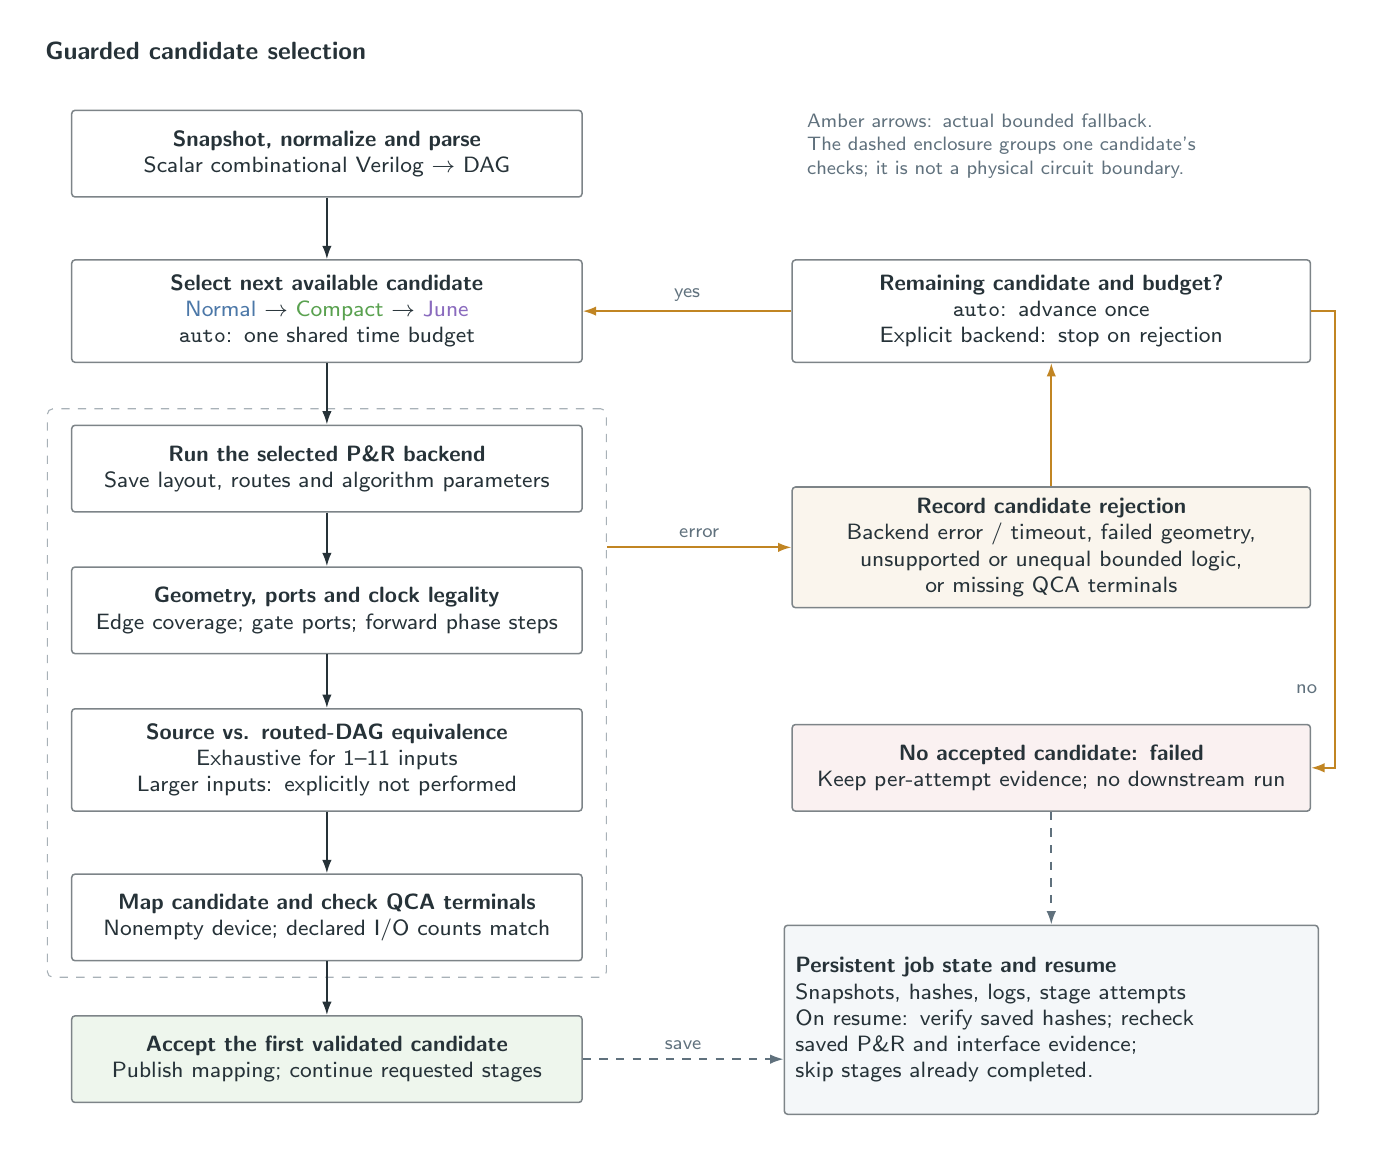
\begin{tikzpicture}[x=1mm,y=1mm]
  \path[use as bounding box] (0,0) rectangle (168,140);
  \node[paneltitle] at (1,137) {Guarded candidate selection};
  \node[box,text width=62mm,minimum height=11mm] (parse) at (38,124)
    {\textbf{Snapshot, normalize and parse}\\Scalar combinational Verilog $\rightarrow$ DAG};
  \node[box,text width=62mm,minimum height=13mm] (select) at (38,104)
    {\textbf{Select next available candidate}\\\textcolor{normal}{Normal} $\rightarrow$ \textcolor{compact}{Compact} $\rightarrow$ \textcolor{june}{June}\\\texttt{auto}: one shared time budget};
  \node[box,text width=62mm,minimum height=11mm] (route) at (38,84)
    {\textbf{Run the selected P\&R backend}\\Save layout, routes and algorithm parameters};
  \node[box,text width=62mm,minimum height=11mm] (geo) at (38,66)
    {\textbf{Geometry, ports and clock legality}\\Edge coverage; gate ports; forward phase steps};
  \node[box,text width=62mm,minimum height=13mm] (logic) at (38,47)
    {\textbf{Source vs. routed-DAG equivalence}\\Exhaustive for 1--11 inputs\\Larger inputs: explicitly not performed};
  \node[box,text width=62mm,minimum height=11mm] (device) at (38,27)
    {\textbf{Map candidate and check QCA terminals}\\Nonempty device; declared I/O counts match};
  \node[box,fill=compact!10,text width=62mm,minimum height=11mm] (accept) at (38,9)
    {\textbf{Accept the first validated candidate}\\Publish mapping; continue requested stages};
  \foreach \a/\b in {parse/select,select/route,route/geo,geo/logic,logic/device,device/accept}
    \draw[flow] (\a.south) -- (\b.north);
  \begin{scope}[on background layer]
    \node[draw=muted!55,dashed,rounded corners=2pt,fit=(route)(geo)(logic)(device),inner xsep=3mm,inner ysep=2mm] (candidate) {};
  \end{scope}
  \node[box,fill=warn!8,text width=63mm,minimum height=14mm] (reject) at (130,74)
    {\textbf{Record candidate rejection}\\Backend error / timeout, failed geometry,\\unsupported or unequal bounded logic,\\or missing QCA terminals};
  \node[box,text width=63mm,minimum height=13mm] (next) at (130,104)
    {\textbf{Remaining candidate and budget?}\\\texttt{auto}: advance once\\Explicit backend: stop on rejection};
  \node[box,fill=bad!8,text width=63mm,minimum height=11mm] (fail) at (130,46)
    {\textbf{No accepted candidate: failed}\\Keep per-attempt evidence; no downstream run};
  \draw[retry] (candidate.east |- reject.west) -- node[smallnote,above,align=center] {error} (reject.west);
  \draw[retry] (reject.north) -- (next.south);
  \draw[retry] (next.west) -- node[smallnote,above] {yes} (select.east);
  \draw[retry] (next.east) -- (166,104) -- (166,46) -- (fail.east);
  \node[smallnote,anchor=east] at (165,56) {no};
  \node[box,fill=grid!30,text width=65mm,minimum height=24mm,align=left] (saved) at (130,14)
    {\textbf{Persistent job state and resume}\\Snapshots, hashes, logs, stage attempts\\On resume: verify saved hashes; recheck\\saved P\&R and interface evidence;\\skip stages already completed.};
  \draw[control] (fail.south) -- (saved.north);
  \draw[control] (accept.east) -- node[smallnote,above] {save} (saved.west |- accept.east);
  \node[smallnote,text width=62mm] at (130,125)
    {Amber arrows: actual bounded fallback.\\The dashed enclosure groups one candidate's\\checks; it is not a physical circuit boundary.};
\end{tikzpicture}
\end{document}
